\documentclass[a4paper,12pt]{article} % Added 12pt for better readability

% Encoding and fonts
\usepackage[T1]{fontenc}
\usepackage{lmodern}
\usepackage{xcolor}      % For color definitions

% Page layout
\usepackage[margin=1in]{geometry}

% Micro-typography
\usepackage{microtype}

% Math packages
\usepackage{amsmath, amssymb, amsthm}

% Graphics and plots
\usepackage{tikz}
\usepackage{pgfplots}
\pgfplotsset{compat=newest}

% Additional utilities
\usepackage{etoolbox}

% Patching pgfplots warning
\usepackage{pgfplots}
\makeatletter
\patchcmd{\pgfplots@applistXXpushback@smallbuf}{\pgfplots@error}{\pgfplots@warning}{}{}
\makeatother

% Theorem and color box settings
\usepackage{tcolorbox}
\tcbuselibrary{theorems}

% Color definitions
\definecolor{custom_green}{HTML}{a3be8c}
\definecolor{custom_red}{HTML}{bf616a}
\definecolor{custom_blue}{HTML}{5e81ac}
\definecolor{blue0}{HTML}{142458}
\definecolor{blue1}{HTML}{186BA1}
\definecolor{blue2}{HTML}{19ABDE}
\definecolor{blue3}{HTML}{1AC9E6}

\definecolor{purple0}{HTML}{29066C}
\definecolor{purple1}{HTML}{7D39C0}
\definecolor{purple2}{HTML}{AF4BCF}
\definecolor{purple3}{HTML}{DA4CB2}

\definecolor{red0}{HTML}{810400}
\definecolor{red1}{HTML}{BF2324}
\definecolor{red2}{HTML}{DE542D}
\definecolor{red3}{HTML}{EF7E32}
% Definition of tcolorboxes
\newtcolorbox{definitionbox}{
  title=Definition,
  fonttitle=\bfseries,
  colback=blue!5!white,
  colframe=blue!30!white,
  coltitle=black,
  boxrule=1.5pt,
  arc=3pt,
  outer arc=3pt,
}

\newtcolorbox{proofbox}{
  title=Proof,
  fonttitle=\bfseries,
  colback=custom_blue!20!white,
  colframe=custom_blue,
  coltitle=white,
  boxrule=0.5pt,
  arc=4pt,
  outer arc=4pt,
}

\newtcolorbox{theorembox}[1][]{
  title={#1},
  fonttitle=\bfseries,
  colback=custom_green!30!white,
  colframe=custom_green,
  coltitle=black,
  boxrule=0.5pt,
  arc=4pt,
  outer arc=4pt,
}

\newtcolorbox{notebox}{
  title=Note,
  fonttitle=\bfseries,
  colback=red!5!white,
  colframe=red!30!white,
  coltitle=black,
  boxrule=0.5pt,
  arc=4pt,
  outer arc=4pt,
}

\newtcolorbox{examplebox}[1][]{
  title=\textbf{Example:} {#1},
  fonttitle=\bfseries,
  colback=custom_red!20!white,
  colframe=custom_red,
  coltitle=white,
  boxrule=0.5pt,
  arc=4pt,
  outer arc=4pt,
}

% Theorem environments
\theoremstyle{definition}
\newtheorem{definition}{Definition}[section]
\newtheorem{example}[definition]{Example}

\theoremstyle{plain}
\newtheorem{theorem}[definition]{Theorem}

% Hyperlinks
\usepackage{hyperref}
\hypersetup{
    colorlinks=true,
    linkcolor=custom_blue,
    urlcolor=custom_blue,
    citecolor=custom_green,
}

% Title and author
\title{
Robert Davidson \\
Complex Analysis Notes
}
\author{
60\% Exam\\
40\% Continuous Assessment (3 parts)
}
\date{} % Empty date

\begin{document}
\maketitle
\pagebreak

\tableofcontents
\pagebreak
\section{Preliminary}
\subsection{The Complex Plane and the Four Quadrants}

The complex plane is a two-dimensional plane where the horizontal axis represents the real part and the vertical axis represents the imaginary part of a complex number. It is divided into four quadrants:

\begin{enumerate}
  \item \textbf{Quadrant I} ($0^\circ < \theta < 90^\circ$): Both $x$ and $y$ are positive.
  \item \textbf{Quadrant II} ($90^\circ < \theta < 180^\circ$): $x$ is negative, $y$ is positive.
  \item \textbf{Quadrant III} ($180^\circ < \theta < 270^\circ$): Both $x$ and $y$ are negative.
  \item \textbf{Quadrant IV} ($270^\circ < \theta < 360^\circ$): $x$ is positive, $y$ is negative.
\end{enumerate}

\hfill

\subsection{Diagram of the Quadrants}
\hfill \hfill 
\begin{center}
  \begin{tikzpicture}[scale=5]
      % Draw axes
      \draw[->] (-1.2,0) -- (1.2,0) node[right] {\text{Re}};
      \draw[->] (0,-1.2) -- (0,1.2) node[above] {\text{Im}};
      
      
      % Label quadrants
      \node at (0.75,0.75) {I};
      \node at (-0.75,0.75) {II};
      \node at (-0.75,-0.75) {III};
      \node at (0.75,-0.75) {IV};
  \end{tikzpicture}
  \end{center}

  \pagebreak

  \subsection{Adjusting Angles Based on Quadrants}

  To correctly determine \( \theta \), adjust the angle returned by \(\tan^{-1}\left(\frac{y}{x}\right)\) according to the quadrant where \( z \) lies.
  
  \begin{enumerate}
      \item \textbf{Quadrant I} (\( x > 0, y > 0 \)):
      \[
      \theta = \tan^{-1}\left(\frac{y}{x}\right)
      \]
      No adjustment needed since \( \theta \) is already between \( 0 \) and \( \frac{\pi}{2} \).
  
      \item \textbf{Quadrant II} (\( x < 0, y > 0 \)):
      \[
      \theta = \pi - \tan^{-1}\left(\frac{y}{|x|}\right)
      \]
      Adjust by subtracting from \( \pi \) to place \( \theta \) between \( \frac{\pi}{2} \) and \( \pi \).
  
      \item \textbf{Quadrant III} (\( x < 0, y < 0 \)):
      \[
      \theta = \pi + \tan^{-1}\left(\frac{|y|}{|x|}\right)
      \]
      Add to \( \pi \) to position \( \theta \) between \( \pi \) and \( \frac{3\pi}{2} \).
  
      \item \textbf{Quadrant IV} (\( x > 0, y < 0 \)):
      \[
      \theta = 2\pi - \tan^{-1}\left(\frac{|y|}{x}\right)
      \]
      Subtract from \( 2\pi \) to set \( \theta \) between \( \frac{3\pi}{2} \) and \( 2\pi \).
  \end{enumerate}

\begin{examplebox}[Let $z = 5 - 2i$]
  $x = 5$ and $y = -2$. Thus, we have:
  $$\theta = 2\pi - \tan^{-1}({2/5}) \approx 338.20^\circ$$
  \begin{center}
    \begin{tikzpicture}[scale=1.5]

      % Draw axes
      \draw[->] (-1, 0) -- (6, 0) node[right] {$\text{Re}$};
      \draw[->] (0, -3) -- (0, 2) node[above] {$\text{Im}$};
  
      % Draw grid (optional)
      \draw[gray, dotted] (-1, -3) grid (6, 2);
  
      % Draw the complex number z = 5 - 2i
      \coordinate (z) at (5, -2);
      \filldraw[red] (z) circle (1.5pt) node[below] {$z = 5 - 2i$};
  
      % Draw the line from origin to z
      \draw[thick, ->] (0, 0) -- (z);
  
      % Draw the angle theta
      \draw[->, custom_red, thick] (0.5, 0) arc (0:338.20:0.5);
      \node[custom_red] at (1,1) {$\theta \approx 338.20^\circ$};
  
      % Label x and y
      \draw[dashed, thin] (5, 0) -- (5, -2);
      \draw[dashed, thin] (0, -2) -- (5, -2);
      \node at (5, 0.3) {$x = 5$};
      \node at (-0.5, -2) {$y = -2$};
  
  \end{tikzpicture}
  \end{center}

\end{examplebox}

\pagebreak
\section{Foundations}
\subsection{Intro to Complex Numbers}
\noindent
\begin{minipage}{0.5\textwidth}
  Complex numbers can be written as the sum of a real and imaginary part:
  $$
  z = x + iy
  $$
  We denote the \textbf{complex conjugate} \((\overline{z})\) as:
  $$
  \overline{z} = x - iy
  $$
  Geometrically, $\overline{z}$ is the \textbf{reflection of z in the real axis}
\end{minipage}\hfill
\begin{minipage}{0.48\textwidth}
  \centering
  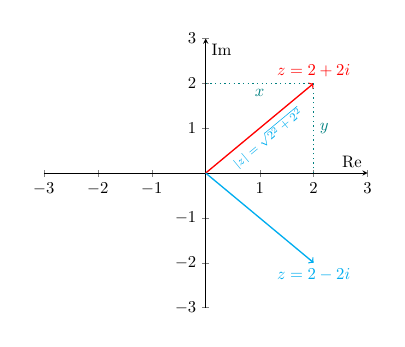
\begin{tikzpicture}[scale=0.6]
    \begin{axis}[
      axis lines = center,
      xlabel = {Re},
      ylabel = {Im},
      xmin = -3, xmax = 3,
      ymin = -3, ymax = 3,
      xtick = {-3,-2,...,3},
      ytick = {-3,-2,...,3},
    ]
      % Red arrow from (0,0) to (2,2)
      \addplot[->, thick, red] 
        coordinates {(0,0) (2,2)}
        node[pos=1, above] {$z = 2 + 2i$}
        node[pos=0.5, sloped, below, cyan, font=\scriptsize] {$|z| = \sqrt{2^2+2^2}$};
      
        \addplot[->, thick, cyan] 
        coordinates {(0,0) (2,-2)}
        node[pos=1, below] {$z =2  - 2i$};


      % Dotted vertical line (labeled y) from (2,0) to (2,2)
      \addplot[dotted, thick, teal] 
        coordinates {(2,0) (2,2)}
        node[midway, right] {$y$};
      
      % Dotted horizontal line (labeled x) from (0,2) to (2,2)
      \addplot[dotted, thick, teal] 
        coordinates {(0,2) (2,2)}
        node[midway, below] {$x$};
      
    \end{axis}
  \end{tikzpicture}
\end{minipage}



\noindent \\ 
With help from Pythagoras' we can now define the distance of $z$ from the origin (\textbf{modulus}), that is the length of the vector pointing to $z$. 
$$|z|^2 = x^2 + y^2 \Rightarrow |z| = \sqrt{x^2 + y^2}$$
We notice that:
\begin{align*}
  z\overline{z} &= (x + iy)(x - iy) \\
  &= x^2 - ixy + ixy - (iy)(iy) \\
  &= x^2 - (i)^2(y^2) \\
  &= x^2 - (-1)(y^2) \\
  &= x^2 + y^2 \\
  &= |z|^2 
\end{align*}
Thus, we have the distance of z from the origin as: $|z| = \sqrt{z\overline{z}} = \sqrt{x^2 + y^2}$
We refer to this as the \textbf{modulus} of $z$ or the \textbf{absolute value} of $z$. \\
Letting $z = x + iy$ and $w = u+iv$, we see:
$$|z -w| = \sqrt{(x-u)^2 + (y-z^2)^2}$$
That is, $|z-w|$ is the distance between $z$ and $w$ in the complex plane. 

\pagebreak

\subsection{Polar Form}

\begin{minipage}{0.48\textwidth}
  Letting \(r = |z| = \sqrt{x^2 + y^2}\), we can define \(x\) and \(y\) as:
  \begin{align*}
    \cos(\theta) &= \frac{x}{r} \quad\Rightarrow\quad x = r\cos\theta, \\
    \sin(\theta) &= \frac{y}{r} \quad\Rightarrow\quad y = r\sin\theta.
  \end{align*}
 
\end{minipage}\hfill
\begin{minipage}{0.48\textwidth}
  \centering
    \begin{tikzpicture}[scale=0.7]
      \begin{axis}[
        axis lines = center,
        xlabel = {Re},
        ylabel = {Im},
        xmin = -3, xmax = 3,
        ymin = -3, ymax = 3,
        xtick=\empty, 
        ytick=\empty,
        clip=false,
      ]
        % Draw the blue vector from (0,0) to (2,2)
        \addplot[->, thick, blue] 
          coordinates {(0,0) (2,2)}
          node[midway, sloped, above, blue] {$r = |z|$}
          node[pos=1, right] {$z = r(\cos\theta + i\sin\theta)$};
        
        % Draw an arc from the positive Re axis to the vector to represent theta.
        \draw[blue, thick] (axis cs:1,0) arc (0:45:1);
        
        % Label the theta angle near the arc.
        \node[blue] at (axis cs:0.5,0.25) {$\theta$};
        
        % Dotted lines representing the x and y components.
        \addplot[dotted, thick, gray] 
          coordinates {(2,0) (2,2)}
          node[midway, right] {$y$};
        \addplot[dotted, thick, gray] 
          coordinates {(0,2) (2,2)}
          node[midway, above] {$x$};
        
      \end{axis}
    \end{tikzpicture}
\end{minipage}
Now:
\begin{align*}
  z &= x + iy \\
    &= r\cos\theta + ir\sin\theta \\
    &= r(\cos\theta + i\sin\theta).
\end{align*}
\noindent To find $\theta$ we usualy calculate $\tan^{-1}(y/x)$ and add/subtract $\pi$, when appropriate. Recalling $\tan^{-1}(y/x) \in (-\pi/2, \pi/2)$.
We denote $\theta$ as  as the \textbf{argument of z}, denoted as $\arg(z)$. Geometrically $\arg(z)$ represent the angle $z$ makes with the positive real axis
Thus, the pair (r, arg(z)) is called the \textbf{polar coordinates of z}. 
We introduce the idea that $\arg(z)$ is a version of Arg$(z)$ that can take multiple values outside of Arg$(z)$'s bounds, ($-\pi, \pi$), more precisely:
$$\arg(z) = \text{Arg}(z) + 2 n \pi, \quad n \in \mathbb{Z}$$

\begin{examplebox}[Find $\text{Arg}(i)$ and $\arg(i)$]
Since $i = 0 + 1i$, we have $x = 0$ and $y = 1$.

Using $\tan^{-1}\left(\frac{y}{x}\right)$:

\[
\arg(z) = \tan^{-1}\left(\frac{1}{0}\right) = \frac{\pi}{2}
\]

Therefore:

\[
\text{Arg}(i) = \frac{\pi}{2}
\]
\[
\arg(i) = \frac{\pi}{2} + 2n\pi, \quad n \in \mathbb{Z}
\]
\end{examplebox}

\pagebreak

\subsection{De Moivre's Theorem}
\textbf{Theorem:} Let $z_1,z_2 \in \mathbb{C}$, be nonzero numbers
$$z_1 = r_1(\cos\theta_1 + i\sin\theta_1) \quad \text{and} \quad z_2 = r_2(\cos\theta_2 + i\sin\theta_2)$$
Then: 
\begin{align*}
  z_1z_2 &= r_1r_2[(cos\theta_1\cos\theta_2  + \sin\theta_1\sin\theta_2) + i(\sin\theta_1\cos\theta_2 + \cos\theta_1\sin\theta_2)] \\
  &= r_1r_2[\cos(\theta_1 + \theta_2) + i\sin(\theta_1 + \theta_2)]
\end{align*}
Thus, we have:
\begin{align*}
  |z_1z_2| &= |z_1||z_2| \\
  \arg(z_1z_2) &= \arg(z_1) + \arg(z_2)
\end{align*}

\begin{theorembox}[Corollary: De Moivre's Theorem]
  Let $n \in \mathbb{Z}$, and $z = |z|(\cos\theta + i\sin\theta)$, then:
  $$z^n = |z|^n = [\cos(n\theta) + i\sin(n\theta)]$$
\end{theorembox}

\subsection{Roots of Unity}
\textbf{Roots of unity are solutions to} $z^n = 1$, where $z$ is a complex number on the unit circle.\\
\textbf{Eulers formula} states that $e^{i\alpha} = \cos\alpha + i\sin\alpha$. \\
Given $z = x+ iy$, then:
$$z = r(\cos\theta + i\sin\theta) = re^{i\theta}$$
Since $z$ lies on the unit circle, we know $R =1$, thus we have 
$$z = e^{i\theta}$$
Also, we can rewrite $1$ as:
\begin{align*}
  1 &= 1 + 0i \\
  &= \cos(0) + i\sin(0) \\
  &= \cos(2\pi) + i\sin(2\pi) \\
  &= \cos(2\pi k) + i\sin(2\pi k) \quad (\text{Periodic with } 2\pi \; \text{so multiples of k don't change the result})\\
  &= e^{i2\pi k} \quad \text{where} \; k \in \mathbb{Z} \quad (\text{By Eulers Formula})
\end{align*}
So we have, $z^n = e^{n(i \theta)}$:
\begin{align*}
  e^{in\theta} &= e^{i2\pi k} \\
  in\theta &= i 2\pi k \\\
  n\theta &= 2\pi k \\
  \theta &= \frac{2\pi k}{n}
\end{align*}
So $\theta$ is the angle corresponding to the $n$-th roots of unity. Using eulers formula again, the solutions are given as:
$$z_k = e_{i\theta} = e^{i(\frac{2\pi k}{n})} = \cos\left(\frac{2\pi k}{n}\right) + i \sin\left(\frac{2\pi k}{n}\right)$$

\pagebreak
\subsection{Complex Roots}
Recall, square roots can be written as $4^{1/2} = \sqrt{4} = 2$, cubic roots as $27^{1/3} = \sqrt[3]{27} = 3$, and so on. Thus, we can write the $n$-th root as $x^{1/n}$. \\
\textbf{What if we wanted to find the $n$-th root of a complex number?} \\
Consider $f(z) = z^{1/n}$, where $n\in \mathbb{Z}$. To solve this, we aim to find some $w$ such that $w^n = z$. \\
Let:
$$z = R[\cos(\theta) + i \sin( \theta)] \quad \text{and} \quad w = r[\cos(\phi) + i \sin(\phi)]$$
From De Moivre's Theorem, we have:
$$w^n = r^n[\cos(n\phi) + i\sin(n\phi)] = R[\cos(\theta) + i\sin(\theta)]$$
We see:
\begin{align*}
  r^n = R &\rightarrow r = \sqrt[n]{R} = R^{1/2} \\
  n\phi = \theta = \theta + 2\pi k &\rightarrow \phi = \frac{\theta}{n} + \frac{2\pi k}{n}\\
\end{align*}
Note that since $\sin$ and $\cos$ are periodic with $2\pi$, the addition of $2\pi k$ doesn't change the result.\\
So we have:
$$z^{1/n} = R^{1/n} [\cos\phi + i \sin\phi]$$
$$\text{with} \quad \phi = \frac{\theta+ 2k\pi}{n}, \quad k \in (0, 1, 2, \dots, n-1)$$
Note that we reserve the notation $\sqrt[n]{z}$ to denote the \textbf{principal root}, defined when $k = 0$.

\begin{examplebox}[Find the cube roots of $z = -1 + i$]
  $R = \sqrt{(-1)^2 + 1^2} = \sqrt{2}$ \\
  We know $z$ is in the second quadrant, so must adjust $\theta$ accordingly: 
  $$\theta = \pi - \tan^{-1}\left(\frac{1}{1}\right) = \pi - \frac{\pi}{4} = \frac{3\pi}{4}$$ 
  We have $k = 0,1,2$ for the cube roots. \\
  Thus, the cubic roots are:
  $$w_k = \sqrt[3]{2} \left[\cos\left(\frac{\theta + 2\pi k}{3}\right) + i\sin\left(\frac{\theta + 2\pi k}{3}\right)\right]$$
\end{examplebox}
\pagebreak
\section{Complex Functions}
\subsection{Trigonemtric Functions}
Recall:
\begin{align*}
  \text{cosine is an even function} &\Rightarrow \cos(-\theta) = \cos(\theta) \\
  \text{sine is an odd function} &\Rightarrow \sin(-\theta) = -\sin(\theta)
\end{align*}
Also recall Eulers formula states $e^{iz} = \cos(z) + i\sin(z) $ also that:
\begin{align*}
  e^{-iz} &= \cos(-z) + i\sin(-z) \\
  &= \cos(z) - i\sin(z) \\
\end{align*}
If we  add these expressions, we get an expression for $\cos(z)$:
\begin{align*}
  e^{iz} + e^{-iz} &= (\cos(z) + i\sin(z)) + (\cos(z) - i \sin(z)) \\
  e^{iz} + e^{-iz}  &= 2\cos(z) \Rightarrow \cos(z) = \frac{e^{iz} + e^{-iz}}{2}
\end{align*}
If we subtract the expressions, we get an expression for $\sin(z)$:
\begin{align*}
  e^{iz} - e^{-iz} &= (\cos(z) + i\sin(z)) - (\cos(z) - i \sin(z)) \\
  e^{iz} - e^{-iz}  &= 2i\sin(z) \Rightarrow \sin(z) = \frac{e^{iz} - e^{-iz}}{2i}
\end{align*}
We can now also derive $\tan(z)$ and $\cot(z)$:
\begin{align*}
  \tan(z) &= \frac{\sin(z)}{\cos(z)} = \frac{\frac{e^{iz} - e^{-iz}}{2i}}{ \frac{e^{iz} + e^{-iz}}{2}} = i \frac{e^{iz} + e^{-iz}}{e^{iz} + e^{-iz}}  \\
  \cot(z) &= \frac{\cos(z)}{\sin(z)} = \frac{\frac{e^{iz} + e^{-iz}}{2}}{\frac{e^{iz} - e^{-iz}}{2i}} = -i \frac{e^{iz} - e^{-iz}}{e^{iz} + e^{-iz}}
\end{align*}

\noindent\textbf{Proposition.} Let $z, z_1, z_2 \in \mathbb{C}$
\begin{align*}
  (i) &\quad \sin(z + 2\pi) = \sin(z)  \quad \text{and} \quad \cos(z + 2\pi) = \cos(z) \\
  (ii) &\quad \cos^2(z) + \sin^2(z) = 1 \\
  (iii) &\quad \sin(z_1 + z_2) = \sin(z_1)\cos(z_2) + \cos(z_1)\sin(z_2) \\
\end{align*}

\subsection{Exponential Functions}
Recall the \textbf{Taylor Series} for $e^x$, that is: $e^x = 1 + x + \frac{x^2}{2!} + \frac{x^3}{3!} + \dots$  \\
We can now define the exponential function for complex numbers as:
$$e^{z} = \sum_{n=0}^{\infty} \frac{z^n}{n!} = 1 + z + \frac{z^2}{2!} +\frac{z^3}{3!} + \dots + \frac{z^n}{n!}$$
Recall also, that $z = re{i\theta} = e^{i\theta}$ it then follows:
$$z = e^{i \theta} = \sum_{n = 0}^{\infty} \frac{(i \theta)^n}{n!} = \underbrace{\left(1 - \frac{\theta^2}{2!} + \frac{\theta^4}{4!} + \dots \right)} _{\cos\theta} + i\underbrace{\left(1 - \frac{\theta^3}{3!} + \frac{\theta^5}{5!} + \dots \right)} _{\cos\theta} = \cos(\theta) + i\sin(\theta)$$

\pagebreak


\subsection{Complex Logarithms}
Recall the log rule: $\log(e^x) = x$. Also recall we defined $\theta = \text{Arg}(z)$ with $\arg(z) = \text{Arg}(z) + 2\pi k$. \\
Lastly, recall the polar form of $z$:
$$z = |z| (\cos(\theta) + i\sin(\theta) ) = e^{i \theta} = |z| e^{i \text{Arg}(z)} = e^{\ln|z| + i \text{Arg} z }$$
We can now define the \textbf{Logarithm of a Complex Number}:
\begin{align*}
  \text{Log}(z) &= \log\left(e^{\ln|z| + i \text{Arg} z }\right) &= \ln|z| + i\; \text{Arg} (z) \\
  \log(z) &= \ln|z| + i \arg z &= \ln|z| + i(\text{Arg}(z) + 2\pi k) 
\end{align*}
\textit{Note:} Denote \text{Log}$(z)$ as the \textbf{principal branch} of the complex logarithm and denote $\log(z)$ as any branch with $k \neq 0$. \\
We can also write the \textbf{Complex logarithm} as:
\begin{align*}
  \log(z) &= \ln|z| + i\arg(z) \\
  &= \ln|z| + i(\text{Arg}(z) + 2k\pi) \\
  &= \ln|z| + i\text{Arg}(z) + 2k\pi i
\end{align*}

\begin{examplebox}[Find the log of $z = 1 + 0i$]
  We have:  \\
    $\circ \;\; z = 1 + 0i = 1  \Rightarrow |z|  = 1$ \\
    $\circ \;\; \text{Arg}(z) = \tan^{-1}{0/1} = 0$ 
    Thus, we have:
    \begin{align*}
      \log(1) &= \ln|1| + i(\text{Arg}(z) + 2k\pi) \\ 
      &= 0 + i(0 + 2k\pi) \\
      &= 2k\pi i \quad \text{where} \; k \in \mathbb{Z}
    \end{align*}
    \begin{center}
      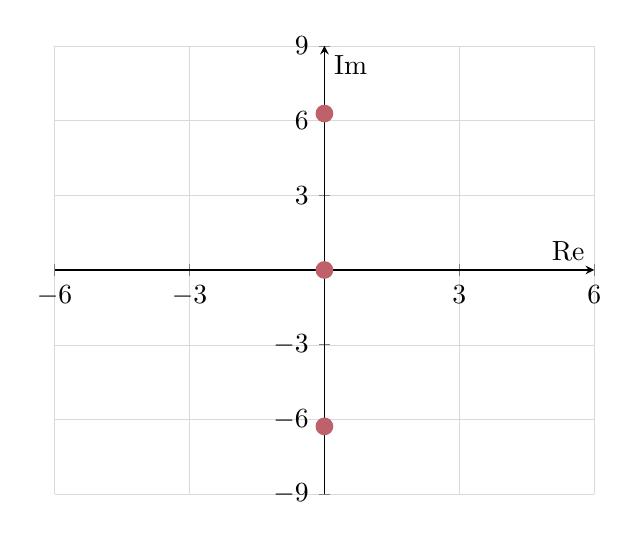
\begin{tikzpicture}[scale = 1]
        \begin{axis}[
          axis lines = center,
          xlabel = {Re},
          ylabel = {Im},
          xmin = -6, xmax = 6,
          ymin = -9, ymax = 9,
          grid = both,
          grid style = {line width=.1pt, draw=gray!30},
          xtick = {-9,-6,...,6,9},
          ytick = {-9,-6,...,6,9},
        ]

        % Plot discrete logarithm values (2kπi)
        \addplot[
          only marks,
          mark = *,
          mark size = 3pt,
          mark options = {custom_red}
        ] coordinates {
          (0, -6.28)
          (0, 0)
          (0, 6.28)
        };

        \end{axis}
      \end{tikzpicture}
\end{center}
\end{examplebox}

\pagebreak

\subsection{Complex Powers}
Recall the Logarithm Rule: $\log(a^b) = b\log(a)$. We want to define $z^\alpha$, in such a way that $\log(z^\alpha) = \alpha \log(z)$. That is the \textbf{Complex Power} is defined as: 
$$z^{\alpha}  = e^{\alpha \log(z)} = e^{\alpha(\text{Log}(z) + 2k \pi i )} \quad \text{for} \, k \in \mathbb{Z}$$
So that we have:
\begin{align*}
  \log(z^\alpha) &= \log(e^{\alpha(\text{Log}(z) + 2k \pi i )}) \\
  &= \alpha(\text{Log}(z) + 2k \pi i) \\
  &= \alpha \log(z)
\end{align*}
As example, consider $z = 1 + 0i$:
\begin{align*}
  1^{\alpha} &= e^{\alpha(Log(1) + 2k \pi i)} \\
  &= e^{2k \alpha \pi i} 
\end{align*}
If $\alpha \in \mathbb{Z}$ $(1,2, 3, \dots)$
$$1^{\alpha} = \left(e^{2k \pi i}\right)^\alpha =  (\cos(2\pi k) + \sin(2\pi k))^\alpha = 1^\alpha = 1$$
If $\alpha = \frac{m}{n} \in \mathbb{Q}$, then $1^\alpha$ is the set of all $n$-th roots of unity:
$$1^{\alpha} = e^{\frac{2k\pi i m}{n}} = \cos\left(\frac{2\pi km}{n}\right) + i \sin\left(\frac{2\pi km}{n}\right) \cos\left(\frac{2\pi r}{n}\right) + i \sin\left(\frac{2\pi r}{n}\right)$$
If $\alpha = i$ then we see:
$$1^\alpha = 1^i = e^{2k\pi i \cdot i} = e^{-2k\pi}$$

\pagebreak

\section{Geomtric Mappings and Transformations}
\subsection{Mappings:}
Recall we defined the principal branch as 
$$\text{Log}(z) = \ln|z| + i \text{Arg}(z)$$
So, when we take the principal branch of the logarithm, we see that it maps to the complex number $w = u + iv$ where $u = \ln|z|$ and $v = \text{Arg}(z)$. \\
In essence. Log maps $\mathbb{C}$ to the horizontal strip:
$$\{w = u+iv: -\pi < v \leq \pi\}$$
\textbf{Diagram of the Logarithm Mapping:} \\
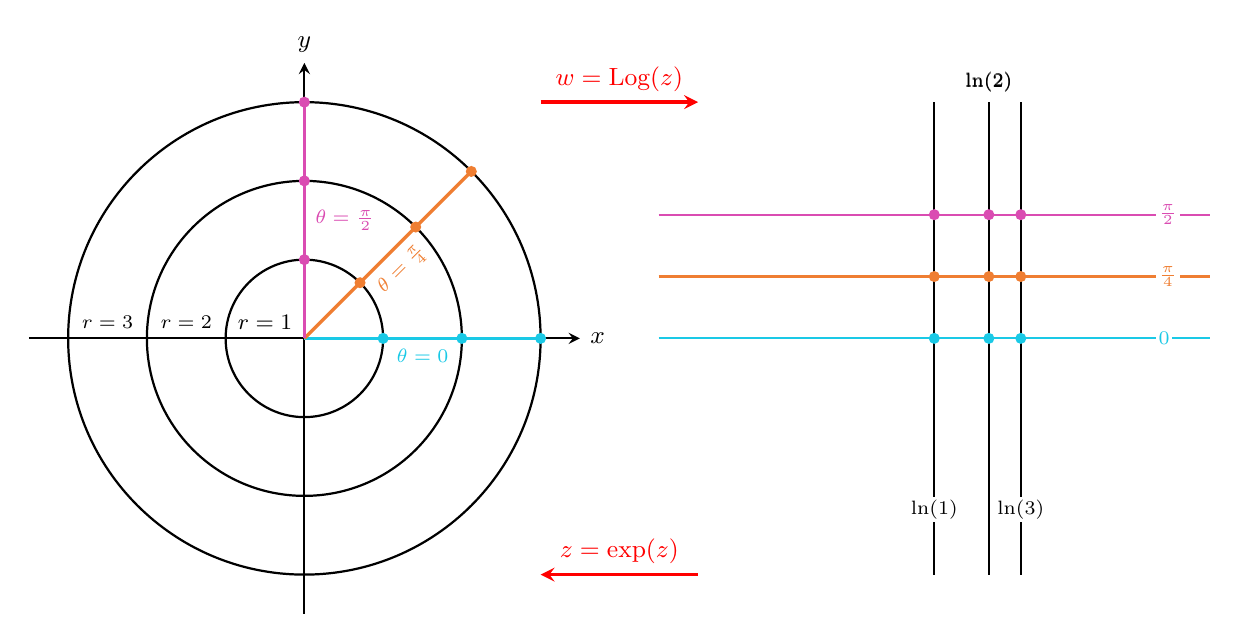
\begin{tikzpicture}[>=stealth, every node/.style={font=\small}, scale =1]

  \draw[->,thick] (-3.5,0) -- (3.5,0) node[right] {$x$};
  \draw[->,thick] (0,-3.5) -- (0,3.5) node[above] {$y$};
  \draw[black, thick] (0,0) circle (1);
  \node[black] at (-0.5,0.2) {\footnotesize$ r = 1$};
  
  \draw[black, thick] (0,0) circle (2);
   \node[black] at (-1.5,0.2) {\scriptsize$ r = 2$};
  \draw[black, thick] (0,0) circle (3);
    \node[black] at (-2.5, 0.2) {\scriptsize$ r = 3$};
  

  
  
  \draw[blue3, very thick] (0,0) -- (3,0) node[midway, below] {\scriptsize$\theta = 0$};
  \draw[red3, very thick] (0,0) -- (2.1213 ,2.1213)  node[midway, below, sloped] {\scriptsize$\theta = \frac{\pi}{4}$};
  \draw[purple3, very thick] (0,0) -- (0,3) node[midway, right] {\scriptsize$\theta = \frac{\pi}{2}$};;;

    \fill[blue3] (1,0) circle (2pt);
    \fill[blue3] (2,0) circle (2pt);
    \fill[blue3] (3,0) circle (2pt);

    \fill[red3] (0.707,0.707) circle (2pt);
    \fill[red3] (1.414,1.414) circle (2pt);
    \fill[red3] (2.12,2.12) circle (2pt);

    \fill[purple3] (0,1) circle (2pt); 
    \fill[purple3] (0,2) circle (2pt);
    \fill[purple3] (0,3) circle (2pt); 

  % Right coordinate system: (u,v) also with (0,0) centered.
  % Shift it horizontally so the two plots appear side by side.
  \begin{scope}[shift={(8,0)}]

    \pgfmathsetmacro{\lnone}{ln(1)}   % ln(1) = 0
    \pgfmathsetmacro{\lntwo}{ln(2)}   % ln(2) ≈ 0.693
    \pgfmathsetmacro{\lnthree}{ln(3)} % ln(3) ≈ 1.099

    % Draw vertical dashed lines at u = ln(1), ln(2), ln(3).
    \draw[dashed, black] (\lnone, -3) -- (\lnone, 3)
      node[pos=0.1667, anchor=north, fill=white, inner sep=1pt] {\scriptsize$\ln(1)$};
    \draw[dashed, black] (\lntwo, -3) -- (\lntwo, 3)
      node[above] {\scriptsize$\ln(2)$};
    \draw[dashed, black] (\lnthree, -3) -- (\lnthree, 3)
      node[pos=0.1667, anchor=north, fill=white, inner sep=1pt] {\scriptsize$\ln(3)$};

      \draw[thick, black] (\lnone, -3) -- (\lnone, 3)
      node[pos=0.1667, anchor=north, fill=white, inner sep=1pt] {\scriptsize$\ln(1)$};
    \draw[thick, black] (\lntwo, -3) -- (\lntwo, 3)
      node[above] {\scriptsize$\ln(2)$};
    \draw[thick, black] (\lnthree, -3) -- (\lnthree, 3)
      node[pos=0.1667, anchor=north, fill=white, inner sep=1pt] {\scriptsize$\ln(3)$};
        
     \draw[thick, blue3] (-3.5,0) -- (3.5,0)
      node[pos=0.9, anchor=west, fill=white, inner sep=1pt] {\scriptsize\(0\)};
    \draw[thick, red3] (-3.5,{pi/4}) -- (3.5,{pi/4})
      node[pos=0.9, anchor=west, fill=white, inner sep=1pt] {\scriptsize\(\frac{\pi}{4}\)};
    \draw[thick, purple3] (-3.5,{pi/2}) -- (3.5,{pi/2})
      node[pos=0.9, anchor=west, fill=white, inner sep=1pt] {\scriptsize\(\frac{\pi}{2}\)};

    \fill[blue3] (\lnone,0) circle (2pt);
    \fill[blue3] (\lntwo,0) circle (2pt);
    \fill[blue3] (\lnthree,0) circle (2pt);

    \fill[red3] (\lnone,{pi/4}) circle (2pt);
    \fill[red3] (\lntwo,{pi/4}) circle (2pt);
    \fill[red3] (\lnthree,{pi/4}) circle (2pt);

    \fill[purple3] (\lnone,{pi/2}) circle (2pt); 
    \fill[purple3] (\lntwo,{pi/2}) circle (2pt);
    \fill[purple3] (\lnthree,{pi/2}) circle (2pt); 
      
    \end{scope}

      

  
  \draw[->, very thick, red] (3,3) -- (5,3)
    node[midway, above,] {$ w= \text{Log}(z)$};

    \draw[<-, very thick, red] (3,-3) -- (5,-3)
    node[midway, above,] {$z= \text{exp}(z)$};

\end{tikzpicture}

\pagebreak

\subsubsection{Example Mapping 1}
Let \( f(z) = z^3 \), we see that: \\[1ex]
\begin{minipage}{0.47\textwidth}
Using exponential rules and polar representation:
  \begin{align*}
    z &= |z|e^{i\theta} \\
    z^3 &= \bigl(|z|e^{i\theta}\bigr)^3 \\
         &= |z|^3 e^{i3\theta} \\
         &= |z|^3 \Bigl(\cos(3\theta) + i\sin(3\theta)\Bigr)
  \end{align*}
\end{minipage}\hfill
\begin{minipage}{0.47\textwidth}
Alternatively, using our definition for complex powers:
  \begin{align*}
    z^3 &= e^{3\log(z)} \\
         &= e^{3\bigl(\ln|z| + i\,\mathrm{Arg}(z)\bigr)} \\
         &= e^{3\ln|z| + i3\,\mathrm{Arg}(z)} \\
         &= |z|^3 e^{i3\,\mathrm{Arg}(z)} \\
         &= |z|^3 \Bigl(\cos(3\theta) + i\sin(3\theta)\Bigr)
  \end{align*}
\end{minipage}\hfill\\[1ex]
Letting $z = 1 + 1i$, we see:
$\theta = \tan^{-1}\left(\frac{1}{1}\right) = 45^\circ = \frac{\pi}{4},$
and $|z| = \sqrt{1^2 + 1^2} = \sqrt{2}$.  Thus, we have: \\
\begin{minipage}{0.47\textwidth}
\begin{align*}
  z^3 &= |z|^3\cdot \left[\cos(3\theta) + i\sin(3\theta)\right] \\
      &= (\sqrt{2})^3\cdot \left[\cos\left(\frac{3\pi}{4}\right) + i\sin\left(\frac{3\pi}{4}\right)\right] \\
      &= 2\sqrt{2}\cdot \left[\cos\left(\frac{3\pi}{4}\right) + i\sin\left(\frac{3\pi}{4}\right)\right] \\
      &= -2\sqrt{2} + i 2\sqrt{2}
\end{align*}
\end{minipage}\hfill
\begin{minipage}{0.47\textwidth}
  \begin{tikzpicture}[scale=1.0, every node/.style={font=\small}]

    % Draw the coordinate axes
    \draw[->] (-3,0) -- (3,0) node[right] {$\text{Re}$};
    \draw[->] (0,-2) -- (0,2) node[above] {$\text{Im}$};
  
    % Plot the complex number z = 1 + i (blue arrow)
    \draw[-, thick, blue3] (0,0) -- (1,1);
    \fill[blue3] (1,1) circle (2pt);
    \node[blue3, above right] at (1,1) {$1+i$};
  
    % Plot the complex number z^3 = -2 + 2i (red arrow)
    \draw[-, thick, red3] (0,0) -- (-2,2);
    \fill[red3] (-2,2) circle (2pt);
    \node[red3, above left] at (-2,2) {$-2+2i$};
  
    % Draw an arc for the angle of z (pi/4)
    \draw[blue3] (1,0) arc (0:45:1);
    \node[blue3, right] at (0.55,0.25) {\scriptsize$\theta$};
  
    % Draw an arc for the angle of z^3 (3pi/4)
    \draw[red3, dashed] (0.65,0) arc (0:135:0.65) node[below, right] {\scriptsize$3\theta$};
  
  \end{tikzpicture}
\end{minipage}\hfill\\
In essence, the mapping $f(z) = z^3$ rotates the complex number $z$ by $3\theta$ and scales it by $|z|^3$.
We can imagine this, for the complex numbers with $|z| = 1$, and $0 < \theta \leq \frac{\pi}{2}$, as an arc of radius $1$, from the angle $0 \to 90^\circ$, mapped to an arc of radius $8$, from the angles $0 \to 270^\circ$.

\pagebreak

\subsubsection{Example Mapping 2}
We wish to find the image of the line \(x=1\) under
\[
f(z)=\frac{1}{z}, \quad z=x+iy, \quad w=u+iv.
\]
For \(z=x+iy\) we have
\[
w=\frac{1}{x+iy}=\frac{x-iy}{x^2+y^2}=\frac{x}{x^2+y^2}-i\frac{y}{x^2+y^2},
\]
so that
\[
u=\frac{x}{x^2+y^2},\quad v=-\frac{y}{x^2+y^2}.
\]
Setting \(x=1\) yields
\[
u=\frac{1}{1+y^2},\quad v=-\frac{y}{1+y^2}.
\]
Since 
\[
|w|^2=u^2+v^2=\frac{1}{1+y^2}=u,
\]
it follows that
\[
u^2+v^2=u \quad\Longrightarrow\quad u^2-u+v^2=0.
\]
Completing the square in \(u\) by adding and subtracting \(\frac{1}{4}\):
\[
u^2-u+\frac{1}{4}+v^2=\frac{1}{4} \quad\Longrightarrow\quad \left(u-\frac{1}{2}\right)^2+v^2=\frac{1}{4}.
\]
Thus, the image of \(x=1\) is the circle
\[
\boxed{\left(u-\frac{1}{2}\right)^2+v^2=\frac{1}{4}},
\]
centered at \(\left(\frac{1}{2},0\right)\) with radius \(\frac{1}{2}\)
\begin{center}
  

  \begin{tikzpicture}[>=stealth, every node/.style={font=\small}, scale =2]

    \draw[->,thick] (-0.5,0) -- (1.5,0) node[right] {$x$};
    \draw[->,thick] (0,-1.5) -- (0,1.5) node[above] {$y$};
    
    \draw[-, thick, blue3] (1, -1.5) -- (1,1.5) node[pos=1, right] {$x=1$};


    % Right coordinate system: (u,v) also with (0,0) centered.
    % Shift it horizontally so the two plots appear side by side.
    \begin{scope}[shift={(5,0)}]
          \draw[->,thick] (-0.5,0) -- (1.5,0) node[right] {$u$};
          \draw[->,thick] (0,-1.5) -- (0,1.5) node[above] {$v$};
      \draw[blue3, thick] (0.5,0) circle (0.5);

      \draw[-, thick] (0.5, -0.1) -- (0.5,0.1) node[pos=-1] {\scriptsize$0.5$};


      \end{scope}

        

    
    \draw[->, very thick, red] (2,-1) -- (4,-1)
      node[midway, above,] {$ w= \frac{1}{z}$};


  \end{tikzpicture}

\end{center}
In general, $f(z) = \frac{1}{z}$ maps circle and lines to circles and lines, respectively.

\pagebreak

\subsection{Circle Preservation Theorem}
Consider the equation:
$$A(x^2 + y^2) + Bx + Cy + D = 0$$
We can we that if $A \neq 0$, then we can divide by $A$:
$$x^2 + y^2 + \frac{B}{A}x + \frac{C}{A}y + \frac{D}{A} = 0$$
Completing the square yields:
$$\left(x + \frac{B}{2A}\right)^2 + \left(y + \frac{C}{2A}\right)^2 = \left(\frac{B^2 + C^2 - 4AD}{4A^2}\right)$$
Thus, if $A\neq 0$, we have a circle with center (-B/2A, -C/2A) and radius $\sqrt{\frac{B^2 + C^2 - 4AD}{4A^2}}$. \\
If $A = 0$, then the equation represents a line:
$$Bx + Cy + D = 0$$
If $D = 0$, the circle or  line contains 0:
$$Bx + Cy + D \mid_{(0,0)} = D = 0$$
\textbf{Why is This Important?}\\[1mm]
Under the inversion $f(z) = \frac{1}{z}$ with $z = x+iy$ and $w = u+iv$, one can show that the general equation

$$A(x^2+y^2) + Bx + Cy + D = 0 \quad \underrightarrow{\text{maps to}} \quad D(u^2+v^2) + Bu - Cv + A = 0.$$

\noindent In this transformed equation:
\begin{itemize}
    \item If the original set does not contain the origin  image is a circle.
    \item If the original set does contain the origin then the equation becomes linear:

    \item If the original set is a line (with \(A=0\)), if it does not pass through the origin, its inversion is a circle that passes through the origin.
\end{itemize}
\noindent\textbf{Examples Illustrating the Inversion Effects} \\
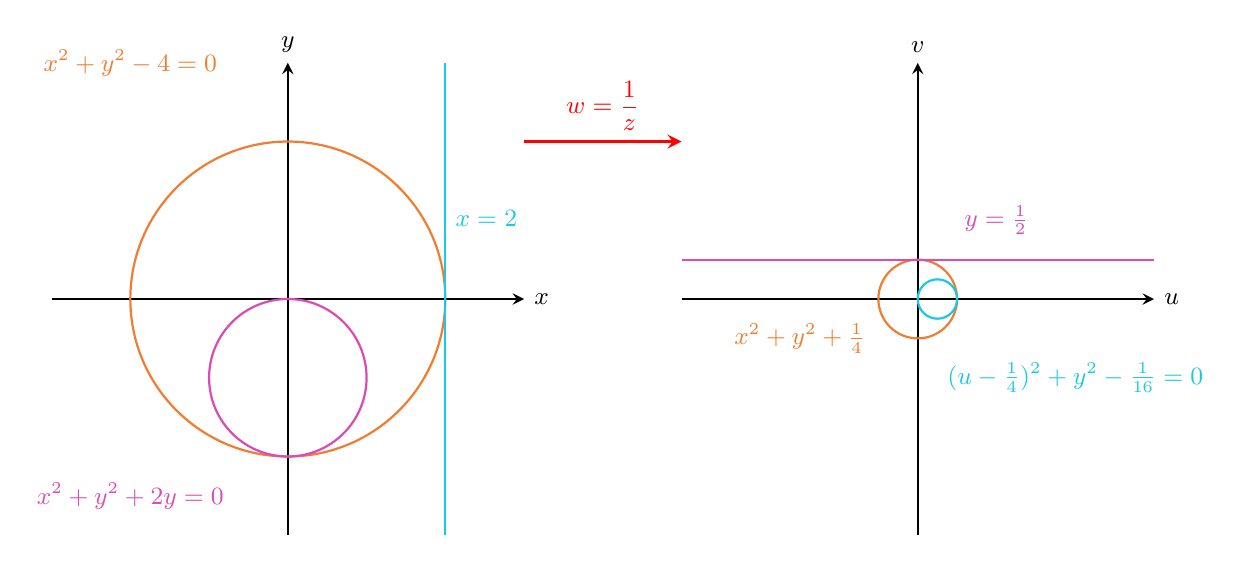
\begin{tikzpicture}[>=stealth, every node/.style={font=\small}, scale =1]

  \draw[->,thick] (-3,0) -- (3,0) node[right] {$x$};
  \draw[->,thick] (0,-3) -- (0,3) node[above] {$y$};
  \draw[red3, thick] (0,0) circle (2);  
  \draw[purple3, thick] (0,-1) circle (1);
  \draw[blue3, thick, -] (2,-3) -- (2,3) node [pos=0.67, right] {$x=2$};

  \node[red3] at (-2,3) {$x^2 + y^2 -4 =0$};
  \node[purple3] at (-2,-2.5) {$x^2 + y^2 + 2y =0$};

\begin{scope}[shift={(8,0)}]

  \draw[->,thick] (-3,0) -- (3,0) node[right] {$u$};
  \draw[->,thick] (0,-3) -- (0,3) node[above] {$v$};

  \draw[red3, thick] (0,0) circle (0.5); 
  \draw[purple3, thick] (-3, 0.5) -- (3, 0.5);
  \draw[blue3, thick] (0.25,0) circle(0.25);

  \node[purple3] at (1,1) {$y = \frac{1}{2}$};
  \node[blue3] at (2,-1) {$(u-\frac{1}{4})^2 +y^2 - \frac{1}{16} = 0$};
  \node[red3] at (-1.5,-0.5) {$x^2 + y^2 + \frac{1}{4}$};
  \end{scope}
  

    


\draw[->, very thick, red] (3,2) -- (5,2)
  node[midway, above,] {$ w= \dfrac{1}{z}$};

  
\end{tikzpicture}
\pagebreak
\subsection{Riemann Sphere}
\subsection{Mobius Transform}
\subsection{Matrix Reprsentation}
\subsection{Cayley Transform}
\end{document} 

